%\documentclass[25pt, a0paper, landscape]{tikzposter}
\documentclass[25pt, a0paper]{tikzposter}
\tikzposterlatexaffectionproofoff
\usepackage[utf8]{inputenc}
\usepackage{authblk}
\usepackage{cite}
\makeatletter
\renewcommand\maketitle{\AB@maketitle} % revert \maketitle to its old definition
\renewcommand\AB@affilsepx{\quad\protect\Affilfont} % put affiliations into one line
\makeatother
\renewcommand\Affilfont{\Large} % set font for affiliations
\usepackage{amsmath, amsfonts, amssymb}
\usepackage{tikz}
\usepackage{pgfplots}
% align columns of tikzposter; needs two compilations
\usepackage[colalign]{column_aligned}
\RequirePackage[nottoc]{tocbibind}


% tikzposter meta settings
\usetheme{Default}
\usetitlestyle{Default}
\useblockstyle{Default}

%%%%%%%%%%% redefine title matter to include one logo on each side of the title; adjust with \LogoSep
\makeatletter
\newcommand\insertlogoi[2][]{\def\@insertlogoi{\includegraphics[#1]{#2}}}
\newcommand\insertlogoii[2][]{\def\@insertlogoii{\includegraphics[#1]{#2}}}
\newlength\LogoSep
%\setlength\LogoSep{-70pt}
\setlength\LogoSep{-160pt}

\renewcommand\maketitle[1][]{  % #1 keys
    \normalsize
    \setkeys{title}{#1}
    % Title dummy to get title height
    \node[inner sep=\TP@titleinnersep, line width=\TP@titlelinewidth, anchor=north, minimum width=\TP@visibletextwidth-2\TP@titleinnersep]
     (TP@title) at ($(-0.5\textwidth+44pt+0.5\titlewidth, 0.5\textheight-\TP@titletotopverticalspace)$) {\parbox{\TP@titlewidth-2\TP@titleinnersep}{\TP@maketitle}};
   % (TP@title) at ($(0, 0.5\textheight-\TP@titletotopverticalspace)$) {\parbox{\TP@titlewidth-2\TP@titleinnersep}{\TP@maketitle}};
    \draw let \p1 = ($(TP@title.north)-(TP@title.south)$) in node {
        \setlength{\TP@titleheight}{\y1}
        \setlength{\titleheight}{\y1}
        \global\TP@titleheight=\TP@titleheight
        \global\titleheight=\titleheight
    };

    % Compute title position
    %\setlength{\titleposleft}{-0.5\titlewidth}
    \setlength{\titleposleft}{-0.5\textwidth+44pt}
    \setlength{\titleposright}{\titleposleft+\titlewidth}
    \setlength{\titlepostop}{0.5\textheight-\TP@titletotopverticalspace}
    \setlength{\titleposbottom}{\titlepostop-\titleheight}

    % Title style (background)
    \TP@titlestyle

    % Title node
    \node[inner sep=\TP@titleinnersep, line width=\TP@titlelinewidth,
    anchor=north, minimum width=\TP@visibletextwidth-2\TP@titleinnersep]
    at (\titleposleft+0.5\titlewidth,0.5\textheight-\TP@titletotopverticalspace)
     %anchor=north, minimum width=\TP@visibletextwidth-2\TP@titleinnersep]
    %at (0,0.5\textheight-\TP@titletotopverticalspace)
    (title)
    {\parbox{\TP@titlewidth-2\TP@titleinnersep}{\TP@maketitle}};

    %\node[inner sep=0pt,anchor=west] 
    %at ([xshift=-\LogoSep]title.west)
    %{\@insertlogoi};

    \node[inner sep=0pt,anchor=west] 
    at ([xshift=\LogoSep]title.east)
    %at ([xshift=\LogoSep]title.east)
    {\@insertlogoii};

    % Settings for blocks
    \normalsize
    \setlength{\TP@blocktop}{\titleposbottom-\TP@titletoblockverticalspace}
}
\makeatother
%%%%%%%%%%%%%%%%%%%%%%%%%%%%%%%%%%%%%


% color handling
\definecolor{TumBlue}{cmyk}{1,0.43,0,0}
%\definecolor{TumBlue}{cmyk}{0.64,0.36,0,0.32}
\colorlet{blocktitlebgcolor}{TumBlue}
\colorlet{backgroundcolor}{white}

% title matter
\title{Kickinect - Torwandschießen}

\author[]{Marcel Brunner}
\author[]{Kevin Bein}
\author[]{Jonas Schulz}
\author[]{Chandramohan Sudar}

\affil[]{Technical University of Munich}

%\insertlogoi[width=15cm]{tum_logo}
\insertlogoii[width=15cm]{tum_logo}


% main document
\begin{document}

\maketitle

\begin{columns}
\column{0.5}{
\block{Game}{
In the game \textit{Torwandschießen}, the player tries to kick a football through two openings in a wall.
One hole is aligned at the bottom left and the other hole is at the top right.
The player has five tries to kick the Ball through either of the two openings and collect points (1 point for the bottom and 3 points for the top hole).
Both holes are just slightly bigger than the diameter of the ball which makes it difficult to hit.
When either of the two holes is hit by the ball, the corresponding points are accredited.
The game ends after five tries.
\\
%\begin{center}
%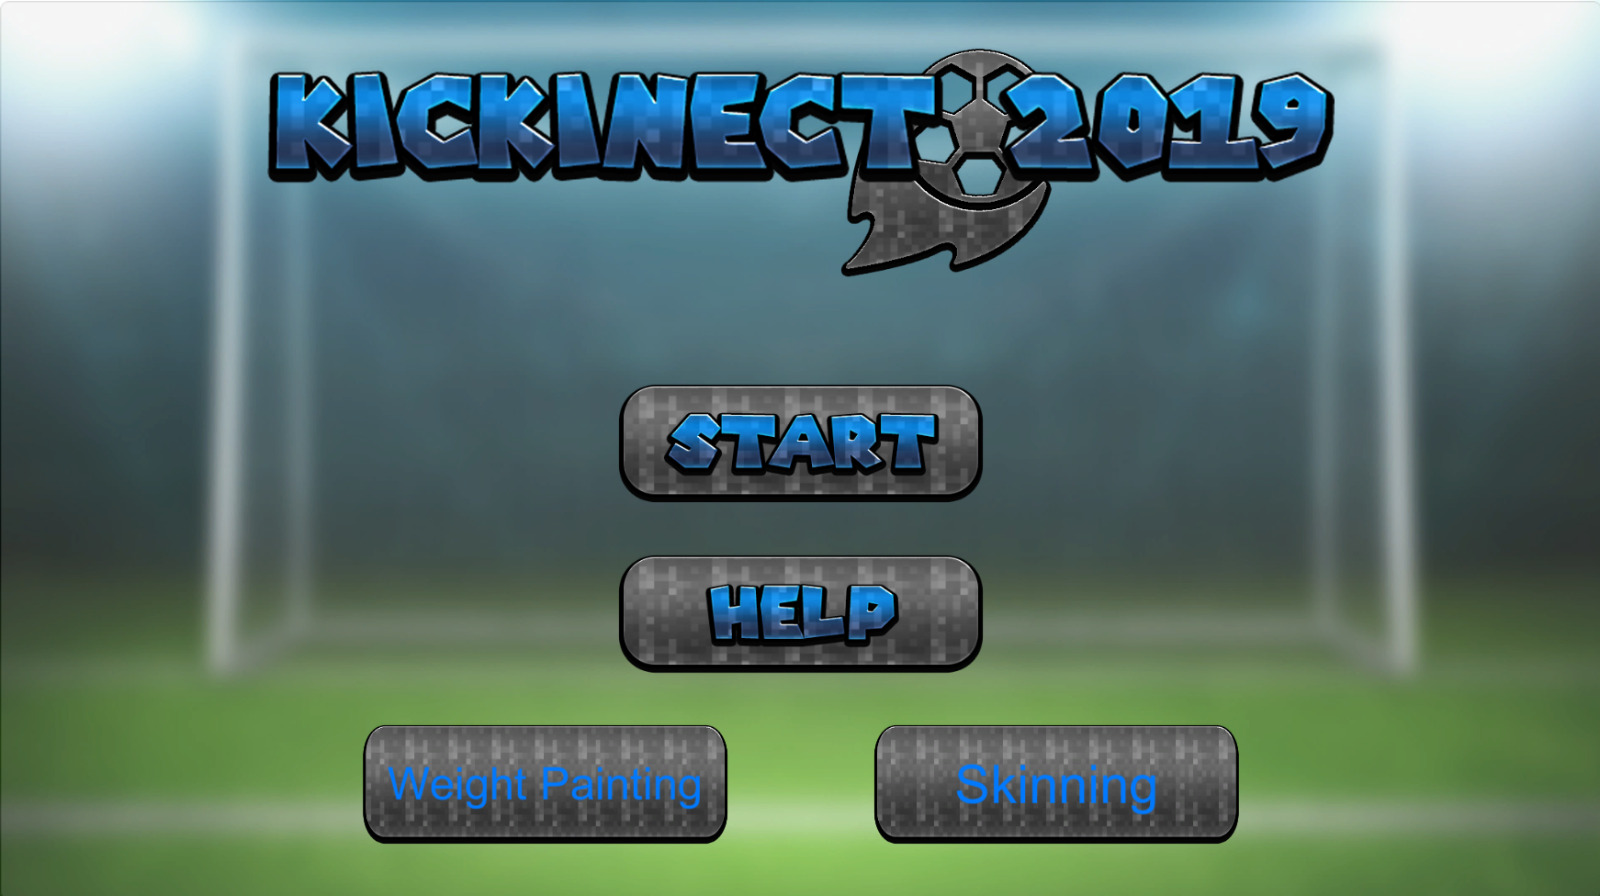
\includegraphics[width=800px]{intro}
%\begin{flushleft}
%\begin{center}
%\textit{Figure 1: Intro}
%\end{center}
%\end{flushleft}
%\end{center}
%\begin{center}
%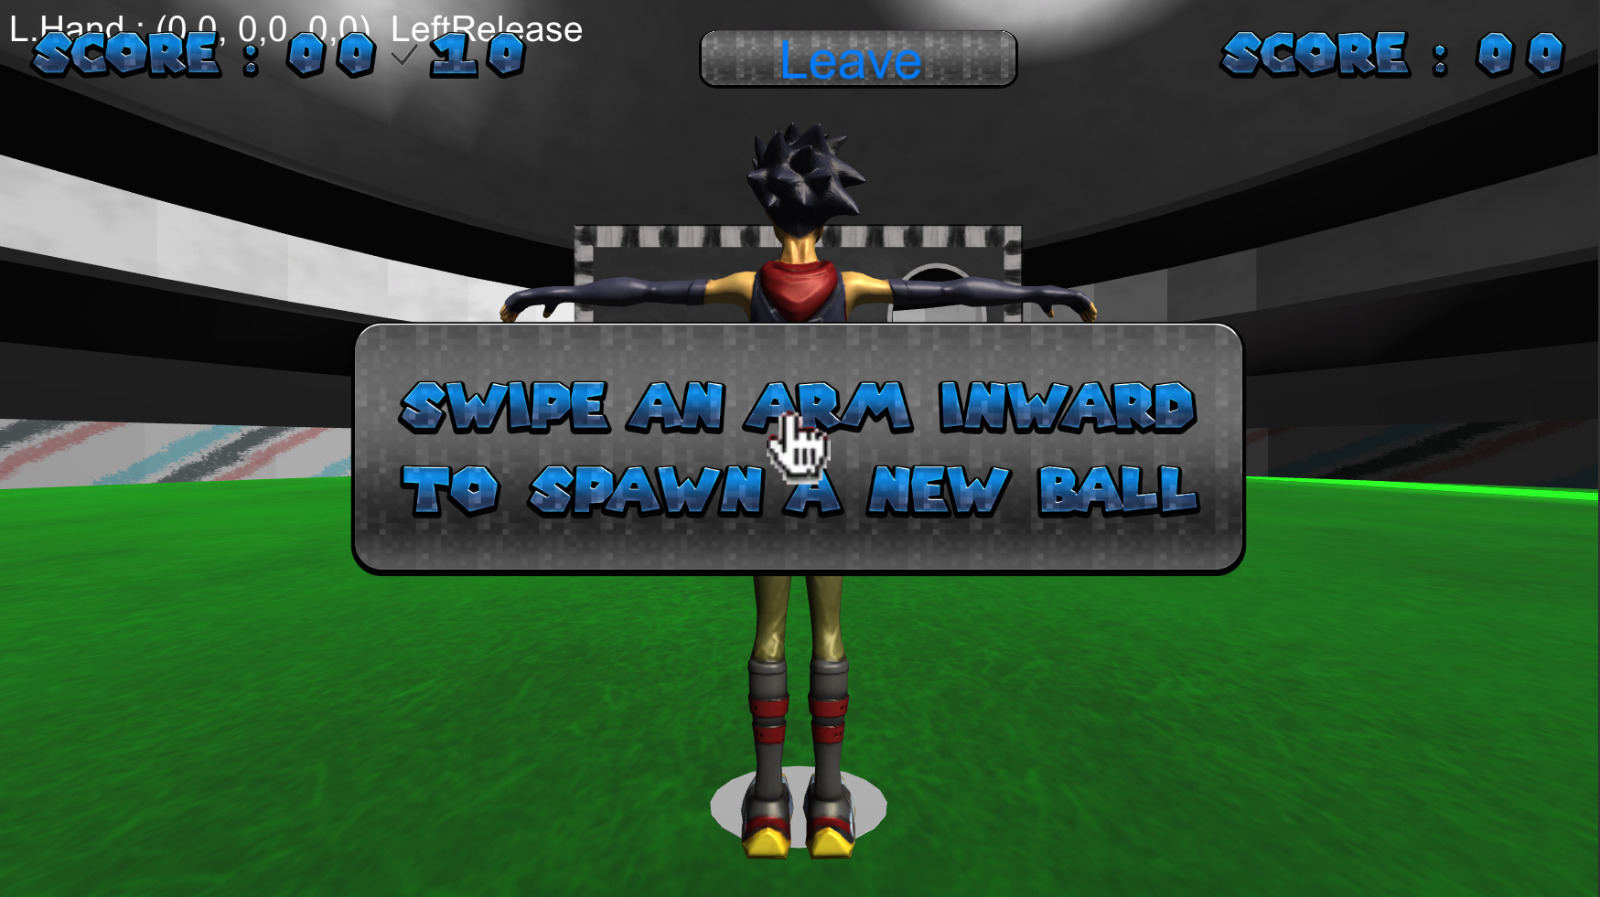
\includegraphics[width=800px]{intro2}
%\begin{flushleft}
%\begin{center}
%\textit{Figure 2: Intro 2}
%\end{center}
%\end{flushleft}
%\end{center}
\begin{center}
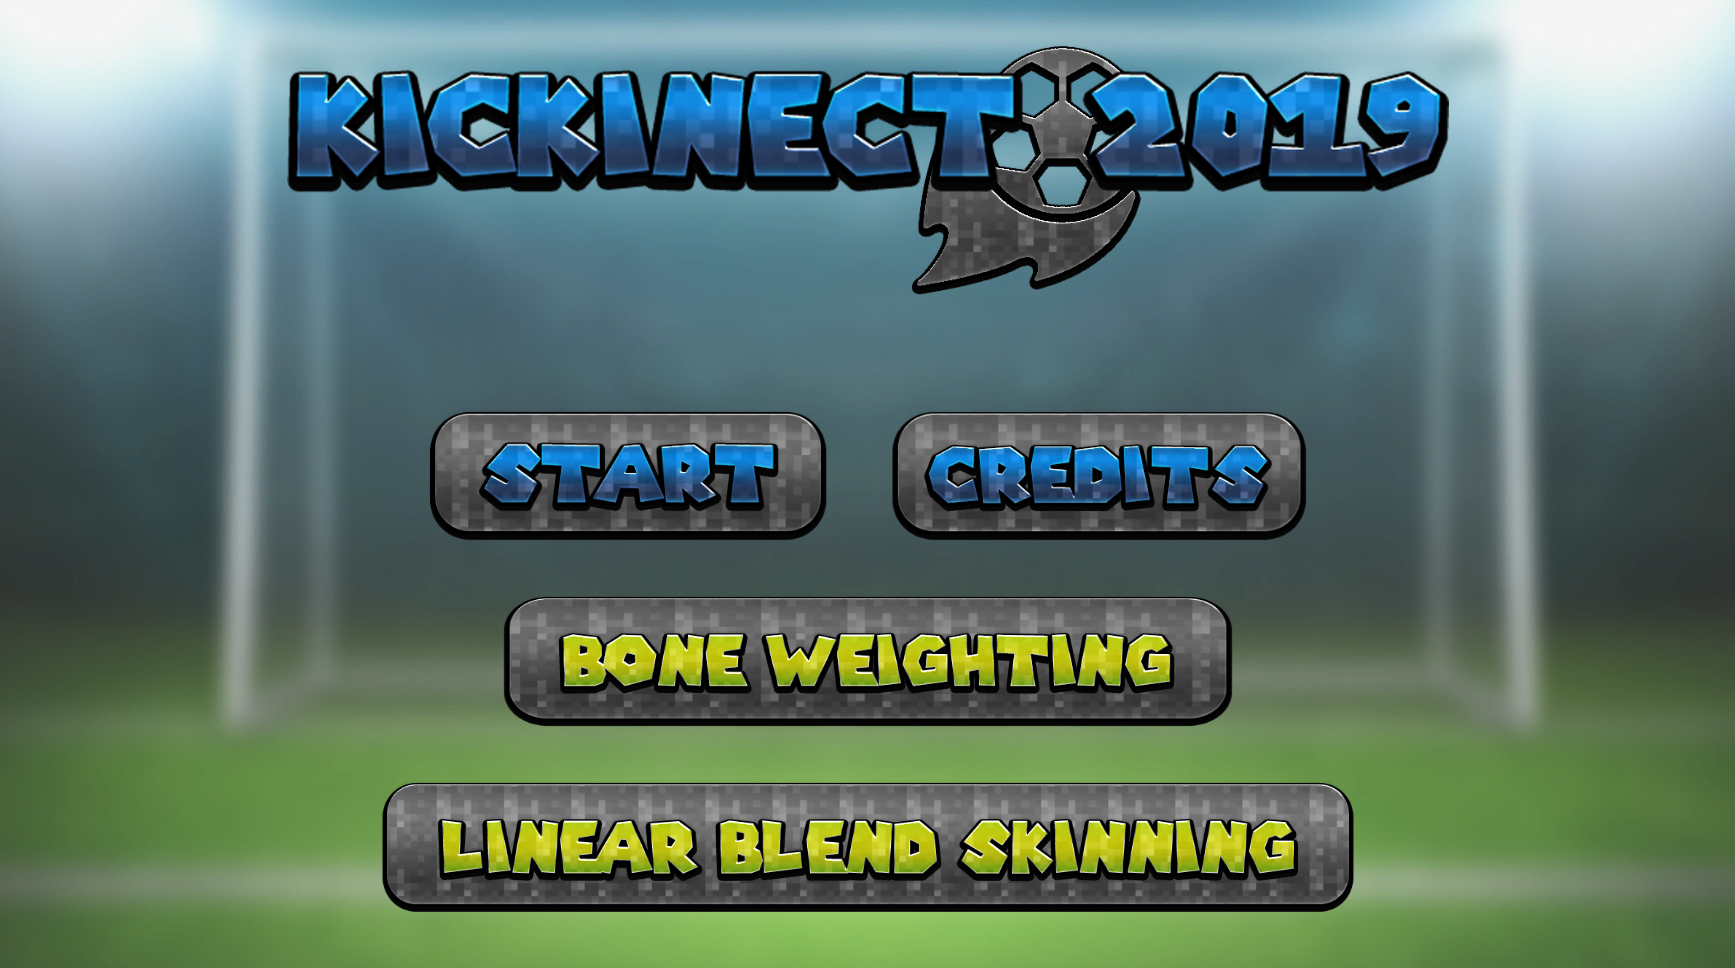
\includegraphics[width=800px]{../Screenshots/intro}
\begin{flushleft}
\begin{center}
\textit{Figure 1: Welcome screen}
\end{center}
\end{flushleft}
\end{center}
}

\block{Linear Blend Skinning}{
Linear blend skinning (\textit{LBS}) is used to deform a mesh by utilizing its skeletal structures.
This is especially interesting to render human body or animal movements.
\textit{LBS} is a very efficient algorithm due to its linear character and as a result can be used for real-time renderings.
The main drawback of this algorithm are bend postures, e.g. armpit distortions.
There are a couple of improvements to basic \textit{LBS} which resolve this problem, most noteworthy is skinning with dual quaternions %\cite{dual_quaternions}
For this project, \textit{LBS} in its basic form is sufficient since only the lower body parts are interesting and these are usually not prone to heavy bending.
\textit{LBS} uses the Rodrigues formula to calculate its rotation matrix
\begin{equation}
\mathrm{R} = e^{\hat{\vec{\omega}}} = \mathrm{I} + \hat{\vec{\omega}} \sin{||\vec{\omega}_j||} + \hat{\vec{\omega}}^2 (1 - \cos{||\vec{\omega}_j})
\end{equation}
which ultimately looks as follows:
\begin{equation}
G(\vec{\omega}, j) = \begin{pmatrix}[e^{\vec{\omega}}]_{3\times 3} & j_{3\times 1} \\ 0_{1\times 3} & 1]\end{pmatrix}
\end{equation}
This rotation matrix is applied linearily to all related body parts along the sceleton structure.
For example, when the leg moves, it directly influences the position of the knee, the feet and the the toes.
Another example is the shoulder: When it moves, it influences the position of the elbow, the hand and the fingers.
Mathematically, this corresponds to chaining $G(\vec{\omega}, j)$:
\begin{equation}
G(\vec{\omega}_1,\vec{\omega}_2,\ldots,\vec{\omega_k}, j_1, j_2, \ldots, j_k) = G(\vec{\omega}_1, j_1) \cdot G(\vec{\omega}_1, j_1) \cdot \ldots \cdots G(\vec{\omega}_k, j_k)
\end{equation}
where $||\vec{\omega}_j||$ is the angle of ration and $\vec{\omega}_j$ is the scaled axis of the rotation.

The $\omega$s are already provided by the Kinect itself as well as the joint locations $J = (j_1, \ldots, j_k)^T$.
Finally, this formula can be applied to the resting pose:
\begin{equation}
\bar{t}_i^\prime = \sum_{k=1}^K \omega_{k,i} G^\prime_k(\vec{theta}, J) \bar{t}_i
\end{equation}

%\begin{center}
%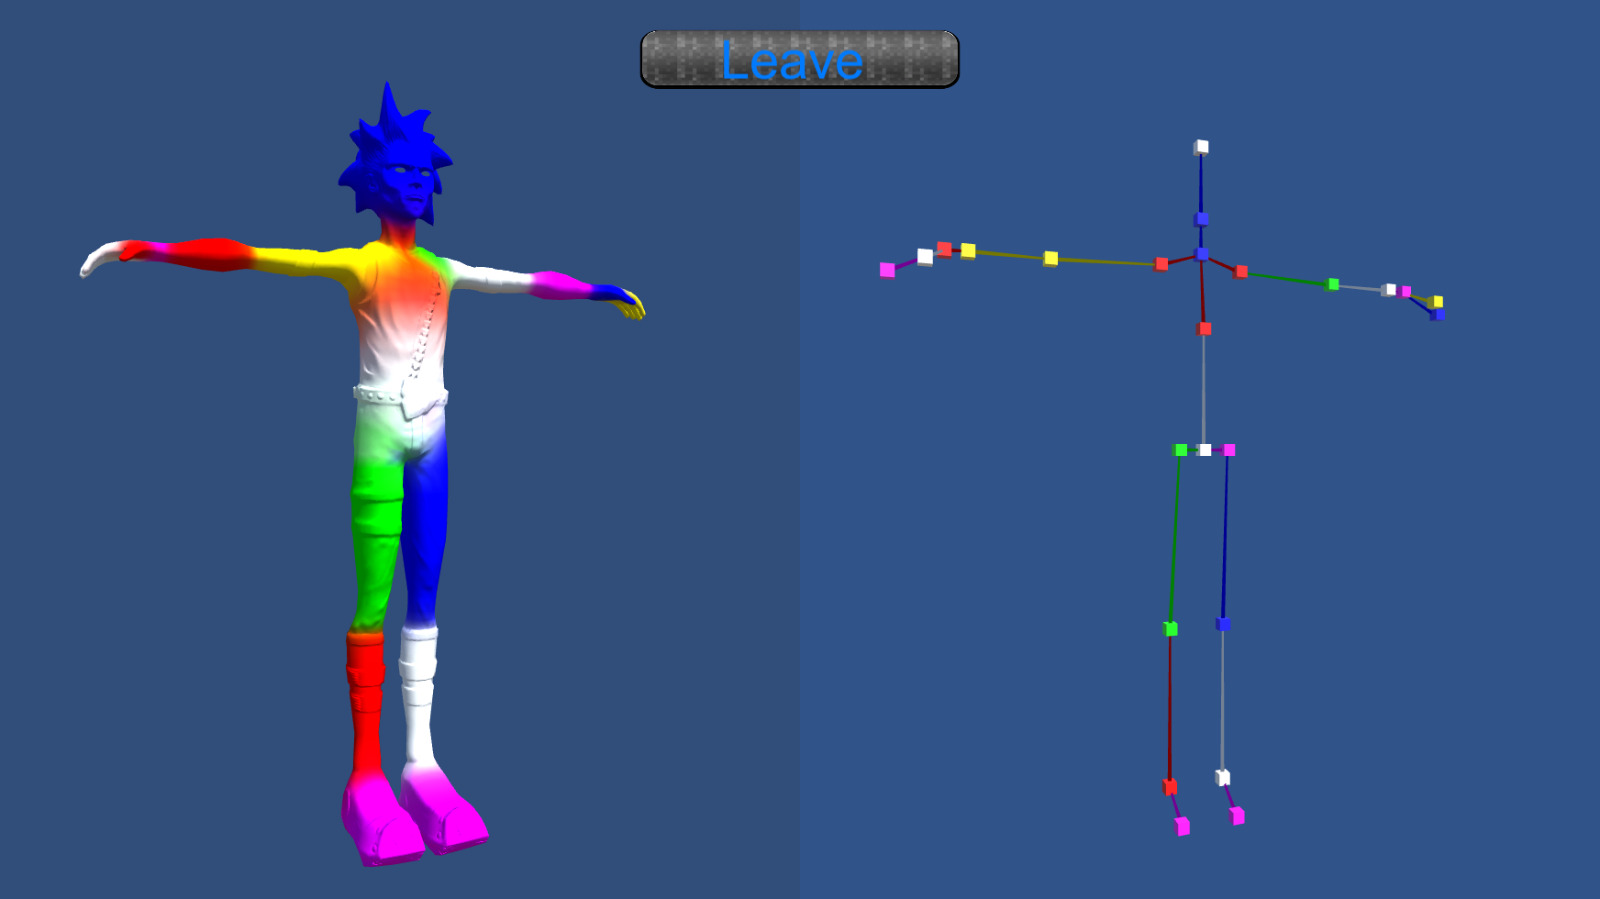
\includegraphics[width=800px]{resting_pose}
%\begin{flushleft}
%\begin{center}
%\textit{Figure 3: Resting pose}
%\end{center}
%\end{flushleft}
%\end{center}

\begin{center}
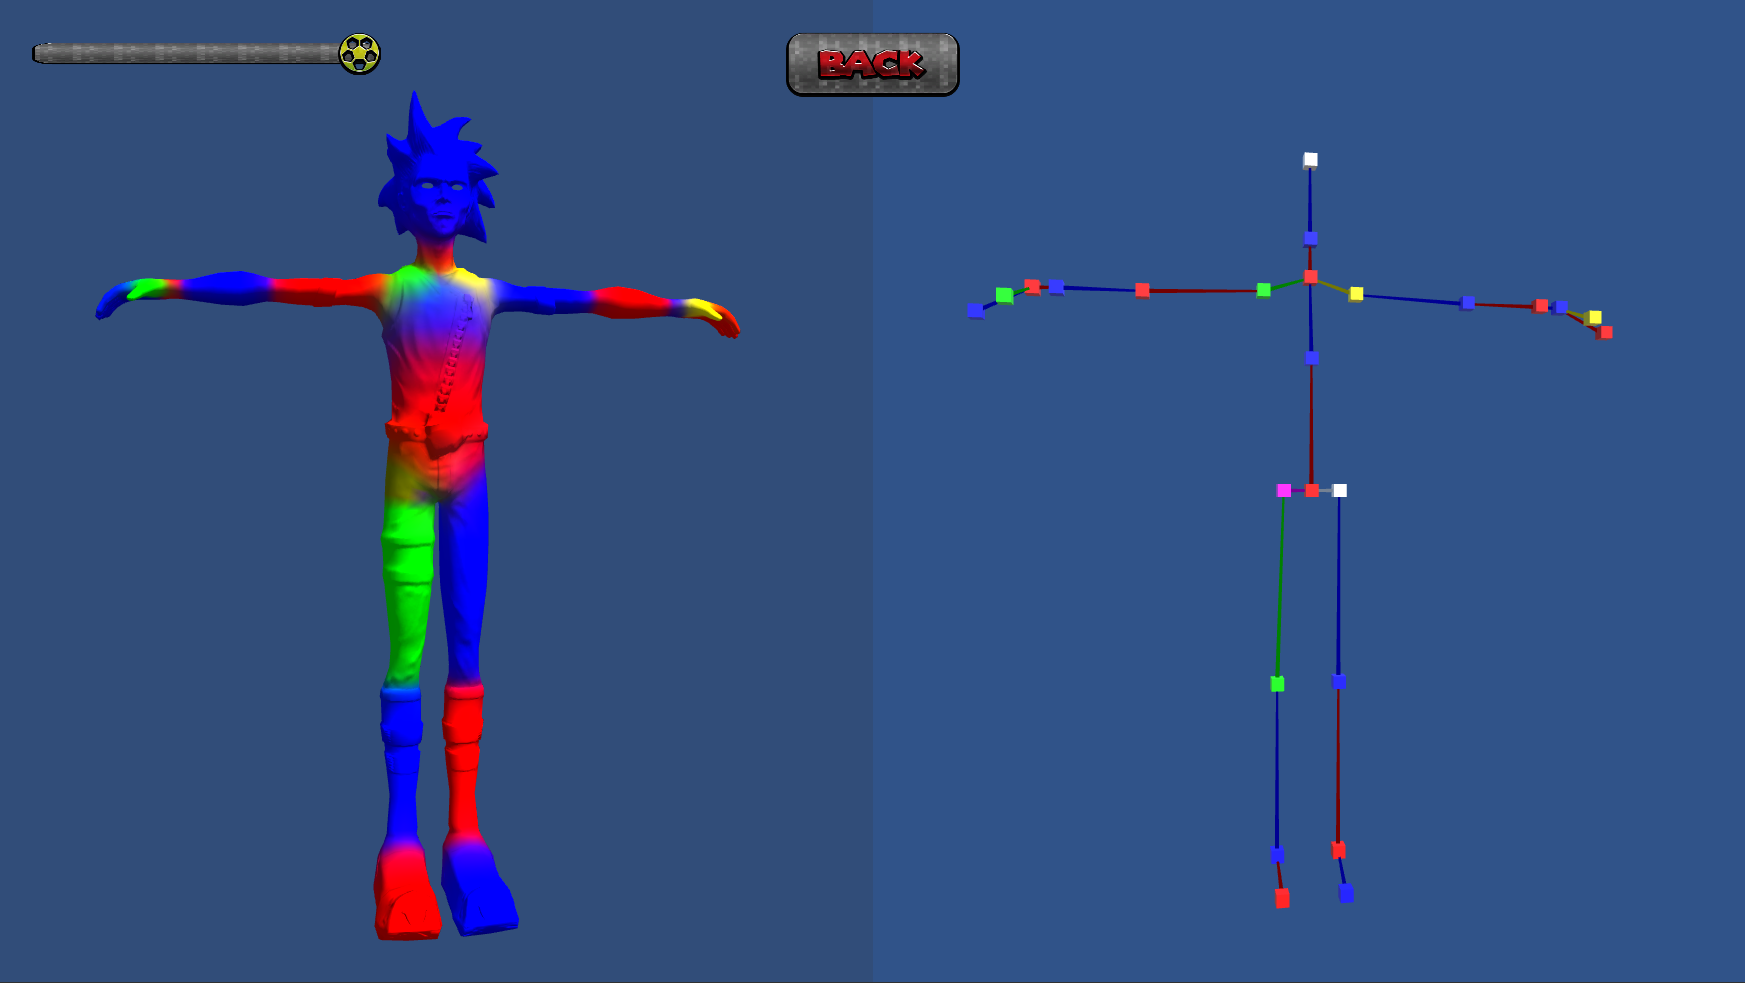
\includegraphics[width=800px]{../Screenshots/weight_colors}
\begin{flushleft}
\begin{center}
\textit{Figure 3: Body weights joints applied to the skeleton and player figure}
\end{center}
\end{flushleft}
\end{center}
}
}


%%\block{Implementation}{
%The setup 
%}
%
%\block{Optimizations}{
%- Hitboxes around the feet to accurately hit the ball
%}
%}

\column{0.5}{
\block{Overview}{
\begin{flushleft}
A Microsoft Kinect Sensor is used to track the player and his movements.
From this input data and the kinect SDK, a body skeleton is calculated and extracted (TODO: figure 2).
By using \textit{Linear Blend Skinning}, this skeleton is mapped onto the 3D Model of a football player in Unity.
For this game, it is especially important to detect movements of the lower body: the player's hips, knees, legs and feet.
With the movement mapped to the model, the only thing left is to construct hitboxes around the players feet.
\end{flushleft}
\begin{flushleft}
The scene consists of the Torwand and a ball, both which are hittable.
Since the implementation of the collision detection and physics calculation are not directly related to this project, we are using Unity's build-in features.
Still, the model parameters, the position of the ball relative to the player, the hitbox sizes and shapes as well as the velocity calculation for when the player hits the ball need to be optimized and tuned manually.
With this setup, the only thing left is for the player to hit the ball with an appropriate angle and accelerate it towards the Torwand.
\end{flushleft}

\begin{center}
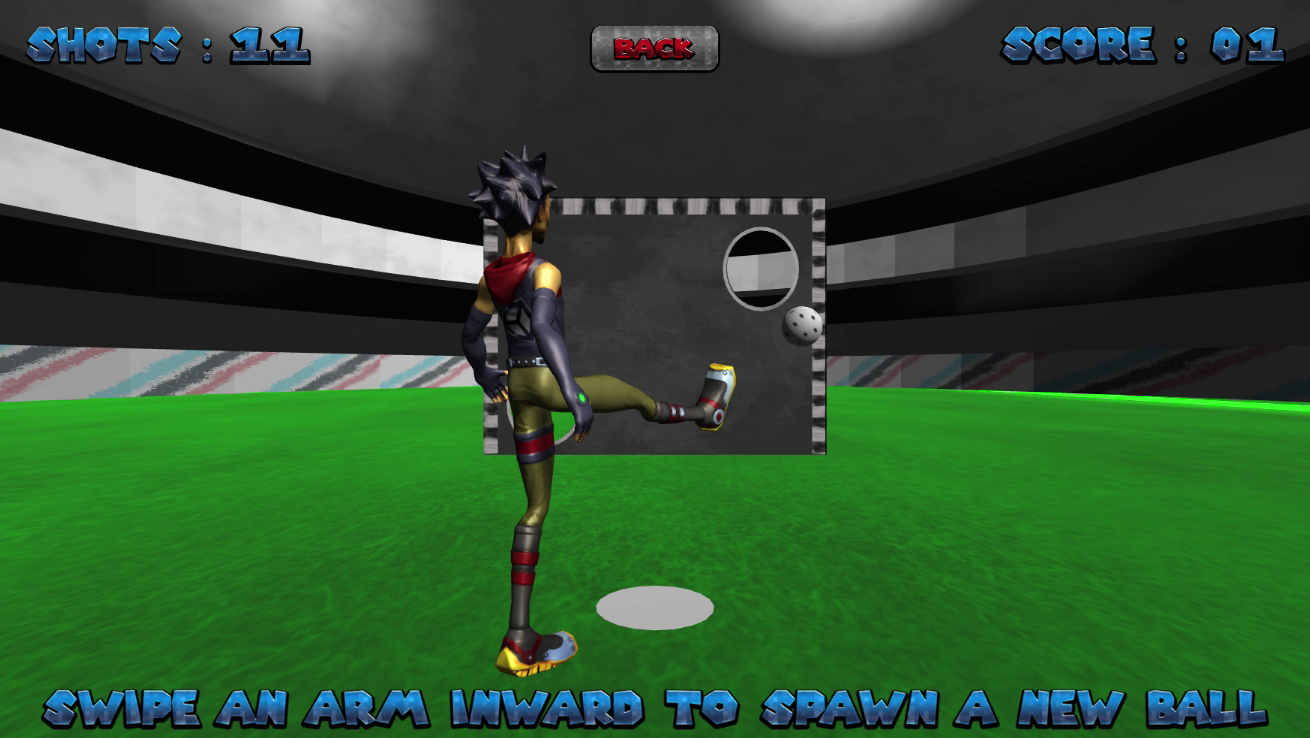
\includegraphics[width=800px]{../Screenshots/main/shooting_scene}
\begin{flushleft}
\begin{center}
\textit{Figure 2: Shooting scene}
\end{center}
\end{flushleft}
\end{center}
}

\block{Challenges}{
\textbf{Ball velocity}

Calculating the velocity with which the ball is accelerated towards the Torwand must be tuned manually.
The following aspects account for a realistic value:
{\begin{enumerate}
  \setlength{\itemsep}{0pt}
  \item The distance of the player to the Torwand
  \item The overall scaling of the scene
  \item The size of the ball in relation to the player
  \item The amount of hitboxes around the players feet as well as their shape
  \item The angle of the hit and the rapidity of the body movement when swinging the foot
  \item The mass of the Ball and the foot
\end{enumerate}}
The first four aspects can be tuned directly in Unity's physics and modle framework by modifying the parameters of the models and rigid bodies.
For the fifth and sixth aspect, applying the formula of an elastic collision yielded very good results:
\[
v = (2 \cdot m_{\text{ball}} \cdot v_{\text{ball}} + (m_{\text{foot}} - m_{\text{ball}}) \cdot v_{\text{foot}}) / (m_{\text{ball}} + m_{\text{foot}})
\]
\\
\textbf{Synchronization}

The biggest challenge comes from synchronizing the Kinect SDK with Unity.
The Kinect is recording an input stream with a depth map and through the SDK, it provides the joints of the body (25 joints in total) and their rotations.
Even though, ultimately, thes values are correct, the joints and rotations do not follow the convention of literature on this topic.

MISSING EXPLANATION
}
}

\end{columns}

\bibliographystyle{plain} 
\bibliography{references}         


\end{document}
